\documentclass[a4paper,10pt]{article}

\usepackage[utf8]{inputenc}             % Encodage du texte (caractères accentués).
\usepackage[french]{babel}              % Langue du document.
\usepackage[sfdefault]{roboto}          % Police d'écriture utilisée dans le document.
\usepackage[T1]{fontenc}                % Règle de césure pour les caractères accentués (pour le compilateur LaTeX).

\usepackage{fancyhdr}                   % Ajout d'en-têtes et de pieds de page à chaque page du document.
\usepackage{graphicx}                   % Ajout d'images dans le document.
\usepackage{hyperref}                   % Création de liens cliquables pointant vers d'autres parties du document.
\usepackage{parskip}                    % Sauts de ligne déterminables entre chaque paragraphe.

% Ne pas oublier de modifier l'option "svgnames" (couleurs définies sur le modèle RGB, meilleur pour
% l'affichage numérique) en option "dvipsnames" (basé sur le modèle de couleur CJMB (CMYK), meilleur
% pour l'impression) via le script de conversion en format imprimable.

\usepackage[usenames,dvipsnames]{xcolor}                    % Coloration du texte.
\usepackage{verbatim}                                       % Mise en page des paragraphes.

\usepackage[document]{ragged2e}                             % Justification du texte.
\usepackage[a4paper,margin=1in,footskip=0.25in]{geometry}   % Mise en page du document.


% ----------------------------------------------------------------------------------------------------------------
% Pour plus d'informations et de documentation sur ces paquets LaTeX, veuillez vous référer aux liens ci-dessous :

% inputenc  : https://www.ctan.org/pkg/inputenc
% babel     : https://www.ctan.org/pkg/babel
% roboto    : https://www.ctan.org/pkg/roboto
% fontenc   : https://www.ctan.org/pkg/fontenc

% fancyhdr  : https://www.ctan.org/pkg/fancyhdr
% graphicx  : https://www.ctan.org/pkg/graphicx
% hyperref  : https://www.ctan.org/pkg/hyperref
% parskip   : https://www.ctan.org/pkg/parskip

% xcolor    : https://www.ctan.org/pkg/xcolor
% verbatim  : https://www.ctan.org/pkg/verbatim

% ragged2e  : https://www.ctan.org/pkg/ragged2e
% geometry  : https://www.ctan.org/pkg/geometry


% ------------------------------------------------------------------------------------------------------------------------
% Liste des couleurs définies (pour la mise en page et pour le changement de thème pour l'impression de la documentation).

% Définition de la couleur       % Normal   | Imprimable    - Description

\definecolor{back}{HTML}{ffffff} % Noir     | Blanc         - Couleur de fond du document.
\definecolor{case}{HTML}{fcff00} % Jaune                    - Couleur des conditions "case".
\definecolor{cmds}{HTML}{909090} % Gris                     - Couleur des noms de commandes du système et de leurs arguments.
\definecolor{cond}{HTML}{be480a} % Brique                   - Couleur des conditions "if".
\definecolor{func}{HTML}{800080} % Mauve                    - Couleur des fonctions définies dans chaque module du framework Bash Utils.

\definecolor{loop}{HTML}{00ffff} % Cyan                     - Couleur des boucles.
\definecolor{main}{HTML}{8F00FF} % Violet                   - Couleur des fonctions du script principal.
\definecolor{path}{HTML}{bfff00} % Citron vert              - Couleur des chemins de dossiers et de fichiers.
\definecolor{sec1}{HTML}{ff0000} % Rouge                    - Couleur des titres principaux et de premier niveau.
\definecolor{sec2}{HTML}{00ff00} % Vert                     - Couleur des titres de deuxième niveau.

\definecolor{sec3}{HTML}{0060ff} % Bleu                     - Couleur des titres de troisième niveau.
\definecolor{text}{HTML}{000000} % Blanc    | Noir          - Couleur du texte normal.
\definecolor{vars}{HTML}{FF7F00} % Orange                   - Couleur des noms des paramètres et des variables.


% ------------------------------------------------------------------------
% Définition de la police d'écriture et de la couleur de fond du document.

\fontfamily{Roboto}

\pagecolor{back}


% ----------------------------------------
% Définition des informations du document.

\title{\color{sec1}Fonctionnement du script\\ \textbf{\color{sec2}256-color-palette.sh}}\color{text}
\author{Dimitri OBEID}
\pagestyle{fancy}

\pdfinfo{
  /Title    (Fonctionnement du script "256-color-palette.sh")
  /Author   (Dimitri OBEID)
  /Creator  (Dimitri OBEID)
  /Producer (Dimitri OBEID)
  /Subject  (Fonctionnement du script "256-color-palette.sh")
  /Keywords ()
}


% ------------------------------------------------------------
% Mise en page des paragraphes et des en-têtes de chaque page.

\setlength{\parskip}{1em}

\setlength{\headheight}{13pt}


% ------------------
% Début du document.

\begin{document}
    \maketitle
    \newpage

    \hypertarget{contents}{}
    \tableofcontents
    \newpage

    \color{sec1}
    \section{Présentation générale du script}\color{text}

    \color{sec2}
    \subsection{Description du script}\color{text}

    \begin{justify}
        Ce script affiche chaque code de couleur de la table de la palette XTERM sur l'arrière-plan du terminal dans un tableau 6 * 40, avec le code correspondant à chaque couleur écrit en trois chiffres au premier plan.
    \end{justify}

    % ------------

    % ----------------------

    % -----------------------------------------------

    \color{sec2}\par\noindent\rule{\textwidth}{0.4pt}\color{text}

    \color{sec2}
    \subsection{Fonctionnement du script}\color{text}

    \begin{justify}
        \textbf{\color{cond}Si} la valeur "-h" ou "--help" est passé en premier argument lors de l'exécution du script, \textbf{\color{cond}alors} un simple message résumant de manière très simple le but du script s'affiche sur le terminal, sans que son code principal, écrit dans la boucle \textbf{\color{loop}for}, elle-même écrite dans la condition alternative, ne s'exécute.
    \end{justify}

    \begin{justify}
        Ce message s'affichera dans les langues suivantes selon la configuration de la variable d'environnement \textbf{\color{vars}\$\{LANG\}}. Il s'affichera en anglais si cette même variable ne stocke pas le code ISO 639-1 relatif à l'une de ces langues :
    \end{justify}

    \begin{justify}
        \begin{itemize}
            \item Allemand, anglais, espagnol, français, indonésien, portuguais, russe, suédois, turc, ukrainien et chinois.
        \end{itemize}
    \end{justify}

    \begin{justify}
    	\textbf{\color{cond}Sinon}, la boucle \textbf{\color{loop}for} suivante est exécutée :

    	\setlength{\parskip}{.3em}

    	\begin{enumerate}
    	    \item \textbf{\color{loop}Tant que} la valeur de la variable \textbf{\color{vars}\$\{i\}}, initialisée à 16 (valeur correspondant au numéro de début de la plage des codes couleurs non-systèmes allant jusqu'au numéro 255 dans la table de couleurs XTERM) est strictement inférieure à 256, \textbf{\color{loop}alors} :

            \begin{enumerate}
                \item La couleur de l'arrière plan du texte est modifiée selon le code couleur correspondant à la valeur de la variable \textbf{\color{vars}\$\{i\}}, puis le numéro à trois chiffres correspondant à cette même valeur est affiché.

                \setlength{\parskip}{1em}

                Voici comment cela fonctionne :

                \begin{itemize}
                    \setlength{\parskip}{1em}

                    \item \textbf{\textbackslash{e}} : Il s'agit du caractère d'échappement (code ASCII 27), qui indique le début d'une séquence d'échappement ANSI.

                    \item \textbf{48}: Il s'agit du code demandant à l'interpréteur Shell de modifier la couleur de l'arrière-plan du texte.

                    \item \textbf{5}: Il s'agit du code indiquant que l'on utilise un index de couleur personnalisé.

                    \item \textbf{\color{vars}\$\{i\}}: La valeur de cette variable est utilisée pour définir le numéro de la table des couleurs XTERM de la couleur spécifique à afficher.

                    \item \textbf{m}: Il s'agit du code de fin de la séquence de contrôle ANSI.
                \end{itemize}

                \setlength{\parskip}{1em}

                \item La mise en forme du texte est supprimée par le biais de la commande \textbf{\color{cmds}printf '\textbackslash{e}[0m'}.

                \item
                {
                    \textbf{\color{cond}Si} l'indice de couleur actuel n'est pas le sixième de la rangée actuelle, \textbf{\color{cond}alors} un espace est écrit pour préparer la prochaine itération de la boucle \textbf{\color{loop}for}, par le biais de la commande \textbf{\color{cmds}printf '\textbackslash{n}'}.

                    \textbf{\color{cond}Sinon}, un saut de ligne est effectué par le biais de la commande \textbf{\color{cmds}printf ' '} pour préparer une nouvelle rangée de six colonnes.
                }

                \item \textbf{\color{cond}Fin de la condition « si »}
            \end{enumerate}

    	\item \textbf{\color{loop}Fin de la boucle « pour »}

    	\end{enumerate}

    	\item \textbf{\color{cond}Fin de la condition « si »}

    \end{justify}

    % ------------

    % ----------------------

    % -----------------------------------------------

    \newpage

    \color{sec2}\par\noindent\rule{\textwidth}{0.4pt}\color{text}

    \color{sec2}
    \subsection{Affichage de la table de palette XTERM sur le terminal}\color{text}

    \begin{justify}
    	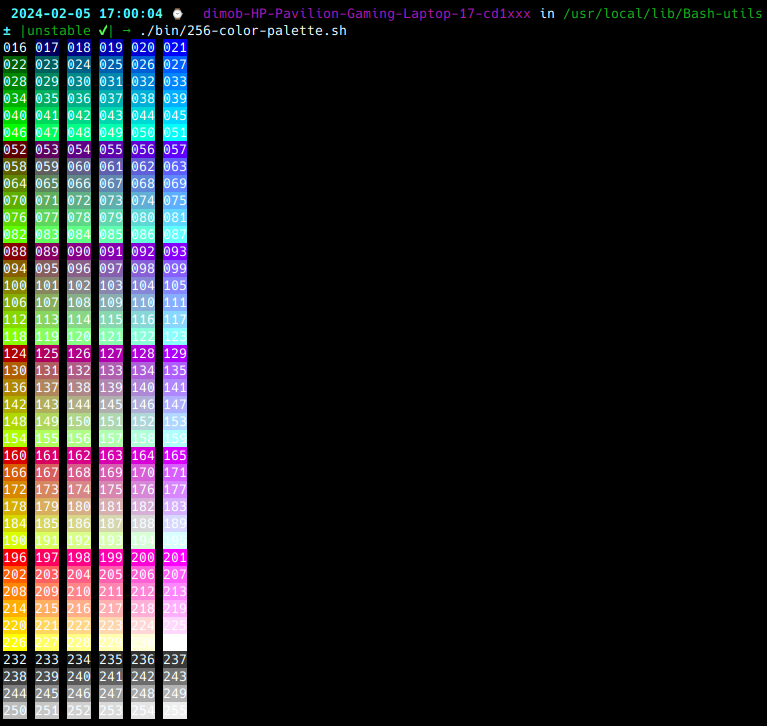
\includegraphics[scale=0.5884]{../../../00 DATA/img/XTERM palette table.png}
    \end{justify}

    % ------------

    % ----------------------

    % -----------------------------------------------

    % /////////////////////////////////////////////////////////////////////////////////////////////// %

\end{document}
